%%%%%%%%%%%%%%%%%%%%%%%%%%%%%%% main.tex %%%%%%%%%%%%%%%%%%%%%%%%%%%%%%%
%                                                                      %
% --------------------- Report Template IST [EN] --------------------- %
%                                                                      %
%       João Marafuz Gaspar                                            %
%       Departamento de Engenharia Eletrotécnica e de Computadores     %
%       Instituto Superior Tecnico                                     %
%       Av. Rovisco Pais                                               %
%       1049-001 Lisboa                                                %
%       Portugal                                                       %
%       E-mail: joao.marafuz.gaspar@tecnico.ulisboa.pt                 %
%                                                                      %
%  Created:       Jul 30, 2022                                         %
%  Last Modified: Apr 6, 2023                                          %
%                                                                      %
%%%%%%%%%%%%%%%%%%%%%%%%%%%%%%%%%%%%%%%%%%%%%%%%%%%%%%%%%%%%%%%%%%%%%%%%
%  Revision history                                                    %
%  v1 - 2022/07/30 - original template                                 %
%  v2 - 2023/04/06 - change superscript in the cover, updated font,    %
%                    added subfigures and table                        %
%%%%%%%%%%%%%%%%%%%%%%%%%%%%%%%%%%%%%%%%%%%%%%%%%%%%%%%%%%%%%%%%%%%%%%%%
%                              Preamble                                %
%%%%%%%%%%%%%%%%%%%%%%%%%%%%%%%%%%%%%%%%%%%%%%%%%%%%%%%%%%%%%%%%%%%%%%%%

% ----------------------------------------------------------------------
% Set the document class
% ----------------------------------------------------------------------
\documentclass[12pt]{article}

% ----------------------------------------------------------------------
% Define external packages, language, margins, fonts, new commands 
% and colors
% ----------------------------------------------------------------------
\usepackage[utf8]{inputenc} % Codification
\usepackage[italian]{babel} % Writing idiom
\usepackage[export]{adjustbox} % Align images
\usepackage{amsmath} % Extra commands for math mode
\usepackage{amssymb} % Mathematical symbols
\usepackage{anysize} % Personalize margins
    \marginsize{2cm}{2cm}{2cm}{2cm} % {left}{right}{above}{below}
\usepackage{appendix} % Appendices
\usepackage{cancel} % Expression cancellation
\usepackage{caption} % Captions
    \DeclareCaptionFont{newfont}{\fontfamily{cmss}\selectfont}
    \captionsetup{labelfont={bf, newfont}}
\usepackage{cite} % Citations, like [1 - 3]
\usepackage{color} % Text coloring
\usepackage{fancyhdr} % Head note and footnote
    \pagestyle{fancy}
    \fancyhf{}
    \fancyfoot[C]{\thepage} % Center of Footnote
    \renewcommand{\footrulewidth}{0.4pt} % Footnote rule
\usepackage{float} % Utilization of [H] in figures
\usepackage{graphicx} % Figures in LaTeX
\usepackage[colorlinks = true, plainpages = true, linkcolor = istblue, urlcolor = istblue, citecolor = istblue, anchorcolor = istblue]{hyperref}
\usepackage{indentfirst} % First paragraph
\usepackage[super]{nth} % Superscripts
\usepackage{siunitx} % SI units
\usepackage{subcaption} % Subfigures
\usepackage{titlesec} % Font
    \titleformat{\section}{\fontfamily{cmss}\selectfont\Large\bfseries}{\thesection}{1em}{}
    \titleformat{\subsection}{\fontfamily{cmss}\selectfont\large\bfseries}{\thesubsection}{1em}{}
    \titleformat{\subsubsection}{\fontfamily{cmss}\selectfont\normalsize\bfseries}{\thesubsubsection}{1em}{}
    \fancyfoot[C]{\fontfamily{cmss}\selectfont\thepage}
\usepackage{minted}
\usepackage{semantic}
\usepackage{url}
\usepackage[T1]{fontenc}
% Random text (not needed)
\usepackage{lipsum}
\usepackage{duckuments}
\usepackage{listings} %For code in appendix
\lstset
{ %Formatting for code in appendix
    language=java,
    basicstyle=\footnotesize,
    numbers=left,
    stepnumber=1,
    showstringspaces=false,
    tabsize=1,
    breaklines=true,
    breakatwhitespace=false,
}

% New and re-newcommands
\newcommand{\sen}{\operatorname{\sen}} % Sine function definition
\newcommand{\HRule}{\rule{\linewidth}{0.5mm}} % Specific rule definition
\renewcommand{\appendixpagename}{\LARGE \fontfamily{cmss}\selectfont Appendices}

% Colors
\definecolor{istblue}{RGB}{3, 171, 230}
\definecolor{dkgreen}{rgb}{0,0.6,0}
\definecolor{gray}{rgb}{0.5,0.5,0.5}


%%%%%%%%%%%%%%%%%%%%%%%%%%%%%%%%%%%%%%%%%%%%%%%%%%%%%%%%%%%%%%%%%%%%%%%%
%                                 Document                             %
%%%%%%%%%%%%%%%%%%%%%%%%%%%%%%%%%%%%%%%%%%%%%%%%%%%%%%%%%%%%%%%%%%%%%%%%
\begin{document}

% ----------------------------------------------------------------------
% Cover
% ----------------------------------------------------------------------
\begin{center}
    \begin{figure}
        \vspace{-1.0cm}
        
\includegraphics[scale = 0.3, center]{Images/logo.png} % IST logo
    \end{figure}
    \mbox{}\\[2.0cm]
    \textsc{\Huge Corso di Complementi di Linguaggi di Programmazione}\\[2.5cm]
    \textsc{\LARGE Report di progetto }\\[2.0cm]
    \HRule\\[0.4cm]
    {\large \bf {\fontfamily{cmss}\selectfont SimpLanPlus}}
    \HRule\\[1.5cm]
\end{center}

\begin{flushleft}
    \textbf{\fontfamily{cmss}\selectfont Gruppo:}
\end{flushleft}

\begin{center}
    \begin{minipage}{0.5\textwidth}
        \begin{flushleft}
            Mae Sosto (0001039236)\\
            Francesco Vece (0001100490)
        \end{flushleft}
    \end{minipage}%
    \begin{minipage}{0.5\textwidth}
        \begin{flushright}
            \href{mailto:mae.sosto@studio.unibo.it}
            {\texttt{mae.sosto@studio.unibo.it}}\\
            \href{mailto:francesco.vece3@studio.unibo.it}
            {\texttt{francesco.vece3@studio.unibo.it}}\\
        \end{flushright}
    \end{minipage}
\end{center}

    
\begin{center}
    \large \bf \fontfamily{cmss}\selectfont 2022/2023 -- 2° Semestre
\end{center}

\thispagestyle{empty}

\setcounter{page}{0}

\newpage

% ----------------------------------------------------------------------
% Contents
% ----------------------------------------------------------------------
\tableofcontents 

\newpage

% ----------------------------------------------------------------------
% Body
% ----------------------------------------------------------------------
\section{Introduzione a SimpLanPlus}
In questo progetto viene sviluppato un compilatore in grado di eseguire SimpLanPlus, un linguaggio imperativo che estende SimpLan \footnote{https://virtuale.unibo.it/pluginfile.php/1550508/mod\_resource/content/1/1.SimpLan\_AND\_ANTLR.pdf}, le sue caratteristiche sono elencate come segue:
\begin{itemize}
\item I tipi ammessi sono: interi, booleani o void.
\item Le dichiarazioni di variabili sono della forma  \textit{type ID} e non ammettono inizializzazione in fase di dichiarazione.
\item Il corpo di una funzione può contenere dichiarazioni e statement, e facoltativamente, possono restituire il valore ottenuto da un'espressione. La dichiarazioni di variabli con lo stesso id è possibile Nel corpo di una funzione è possibile accedere a variabili globali e chiamare altre funzioni, se precedentemente dichiarate. Inoltre, è possibile dichiarare una funzione all'interno del corpo di una funzione (se questa non hanno lo stesso id) ed è possibile avere funzioni ricorsive, ma non mutuamente ricorsive.
\end{itemize}

Il codice utilizzato per lo sviluppo del progetto è disponibile nella repository GitHub nel link a piè di pagina \footnote{}.

\subsection{Grammatica di SimpLanPlus}
In questa sezione vengono evidenziate le differenze e i cambiamenti effettuati tra la grammatica fornita inizialmente e quella effettivamente utilizzata in questo progetto con lo scopo di raggiungere gli obiettivi e le specifiche preposte. Segue grammatica SimpLanPlus.

Al fine di rispettare i requisiti del linguaggio, la grammatica è stata modificata introducendo gli elementi \textit{stms: (stm)+;} e \textit{stme: (stm)* exp;} in modo tale da differenziare i contenuti dei blocchi then e else in entrambi i tipi di if. Più nel dettaglio, l'if presente nell'elemento \textit{stm} diventa \textit{'if' '(' exp ')' '{' left=stms '}' ('else' '{' right=stms '}')?} e l'if presente nell'elemento \textit{exp} diventa \textit{'if' '(' cond=exp ')' '{' left=stme '}' 'else' '{' right=stme '}'}.

Nelle produzioni dell'elemento \textit{exp} sono state aggiunte delle "etichette" che permettono di semplificare i controlli sugli elementi presenti nella produzione. Tali etichette sono \textit{leftExp}, \textit{op} e \textit{rightExp}. Le stesse notazioni sono usate negli elementi riguardanti gli if condizionali. 

Inoltre, per avere maggiore controllo su possibili errori sintattici, è necessario aggiungere in coda al programma in input la notazione \textit{EOF} (end of file).

Per finire, sono state aggiunte delle notazioni sotto forma di \textit{\#notazione} per ogni produzione di ogni elemento che contiene più produzioni per semplificare la gestione di tali produzioni e creare le funzioni necessarie nel visitor. 

%\noindent\fbox{%
%    \parbox{\textwidth}{%
%\lstinputlisting[language=java]{./Code/SimpLanPlus.java}
%}%
%}

\begin{minted}[xleftmargin=20pt,linenos]{antlr}
grammar SimpLanPlus ;
prog   : exp EOF                     #expProg
       | (dec)+ (stm)* (exp)?  EOF   #letProg
       ;
dec    : type ID ';'              #varDec
       | type ID '(' ( param ( ',' param)* )? ')' '{' body '}' #funDec
       ;
param  : type ID
       ;
body   : (dec)* (stm)* (exp)?
	   ;
type   : 'int'
       | 'bool'
       | 'void'
       ;
stm    : ID '=' exp ';' #asgStm                                                                  
       | ID '(' (exp (',' exp)* )? ')' ';'#callStm
       | 'if' '(' exp ')' '{' left=stms '}' ('else' '{' right=stms '}')? #ifStm
	   ;
stms   : (stm)+
       ;
stme   : (stm)* exp
       ;
exp    :  INTEGER #intExp
       | ('true' | 'false') #boolExp
       | ID #idExp
       | '!' exp #notExp
       | leftExp=exp (op='*' | op='/') rightExp=exp #numExp
       | leftExp=exp (op='+' | op='-') rightExp=exp #numExp
       | leftExp=exp  '==' rightExp=exp #eqExp
       | leftExp=exp (op='>' | op='<' | op='>=' | op='<=' ) rightExp=exp #compExp
       | leftExp=exp (op='&&' | op='||') rightExp=exp #opExp
       | 'if' '(' cond=exp ')' '{' left=stme '}' 'else' '{' right=stme '}' #ifExp
       | '(' exp ')' #baseExp
       | ID '(' (exp (',' exp)* )? ')' #callExp
       ;

\end{minted}

\subsection{Struttura compilatore}
Lo schema utilizzato per la stuttura del compilatore è stata costruita su modello della struttura utilizzata per SimpLan, dove: 
\begin{itemize}
    \item \textbf{ast}: contiene le implementazioni dei nodi dell'albero sintattico e dei visitor 
    \item \textbf{evaluator}: contiene le implementazioni per eseguire il codice assembly generato
    \item \textbf{mainPackage}: contiene il main del compilatore, il file del codice in input e del codice assembly generato
    \item \textbf{parser}: contiene le classi generate da ANTLR sulla base della grammatica SimpLanPlus. 
    \item \textbf{svm}: contiene le classi generate da ANTLR sulla base della grammatica SVM.
    \item \textbf{symboltable}: contiene le classi che servono a gestire la symbol table.
    \item \textbf{utils}: contiene le classi utilizzate come supporto alla gestione delle strutture utilizzate.
    
\end{itemize}

\subsection{Software e tools}
Il codice di questo elaborato è stato implementato usando come IDE IntelliJ IDEA \footnote{https://www.jetbrains.com/idea/} sviluppato da JetBrains, un ambiente di sviluppo integrato scritto in Java per lo sviluppo di software scritto in Java. Per quanto riguarda il versioning, è stato utilizzato GitHub, Inc. \footnote{https://github.com} sviluppato da Microsoft Corporation, un servizio di hosting per lo sviluppo di software e il controllo del versioning tramite Git. 
Per la generazione del parser, è stato utilizzato il software ANTLR \footnote{https://www.antlr.org} (ANother Tool for Language Recognition), un generatore di parser che utilizza un algoritmo per il parsing LL.

La versione di Java utilizzata come SDK è la \textit{11.0.18} scaricabile al link \footnote{https://www.oracle.com/java/technologies/javase/11-0-18-relnotes.html} a fondo pagina.
L'unica libreria importata è la seguente \textit{antlr-4.12.0-complete.jar}, anche questa scaricabile gratuitamente tramite il link \footnote{https://www.antlr.org/download.html} a fondo pagina. 



\section{Esercizio 1}
Una volta effettuate le modifiche alla grammatica SimpLanPlus fornita come modello, è stato utilizzato ANTLR per generare il codice utilizzato dal parser e dal lexer. 

Nel main è stato definito il file \textit{prova.simplan} da utilizzare per passare il programma in input e sono stati definiti gli oggetti che gestiscono il parser e il lexer. La libreria di ANTLR ha permesso di utilizzate la classe \textit{ANTLRInputStream} per ottenere il contenuto del file di input, estrarre i token e effettuare il parsing.

In questa fase sono stati definiti tutti gli elementi (appartenenti all'interfaccia \textit{Node}) che fanno parte della grammatica per andare a costruire l'AST (albero di sintassi astratta). Sempre per questo scopo, è stato effettuato un override dei metodi predefiniti contenuti nella classe \textit{SimpLanPlusBaseVisitor}. Questi nuovi metodi si trovano in \textit{SimpLanPlusBaseVisitorImpl} contenuto nel pacchetto \textit{ast} e vengono utilizzati per costruire l'AST nel momento in cui nel main viene chiamata la funzione \textit{visit ()}. 

È stata inoltre implementata la funzione \textit{toPrint()} in tutti i nodi, questa è in grado di stampare sul terminale di IntelliJ l'AST del programma per avere una rappresentazione visiva più chiara.

Per quanto riguarda la gestione degli errori, è in questa fase che è stata implementata la classe \textit{ParserErrorHandler} contenuta nel pacchetto parser per gestire gli errori lessicali e sintattici.
Alla verifica di uno o più errori, l'handler verrà triggerato in modo automatico, le funzioni presenti in \textit{ParserErrorHandler} permetteranno di salvare all’interno di un ArrayList di stringhe gli errori lessicali e sintattici, tali errori verrano scritti nel file \textit{errori.log} presente nel pacchetto mainPackage. La classe \textit{ParserErrorHandler} estende la classe base di ANTLR \textit{BaseErrorListener}, eseguendo l’override del metodo \textit{syntaxError}.

\subsection{Esempi}
Vengono di seguito mostrati tre diversi esempi di codice errati che contengono corrispondentemente un errore lessicale, sintattico e semantico. Tali errori vengono scritti nel file \textit{errori.log}, che si aggiorna ogni volta che un nuovo programma viene eseguito.

\begin{itemize}
\item Il primo tipo di errore trattato è quello lessicale. Questo avviene quando il lexer non è in grado di riconoscere nella stringa di ingresso gruppi di simboli che corrispondono a specifiche categorie sintattiche. Consideriamo il seguente codice e errore riportato dal compilatore SimpLanPlus :
\begin{minted}[xleftmargin=20pt,linenos]{java}
int a;
int 1b;
\end{minted}
\begin{minted}[xleftmargin=20pt, linenos]{java}
[!] An error occurred at line 2, character 4 :no viable alternative at
input 'int1'
[!] An error occurred at line 2, character 5 :mismatched input 'b' 
expecting {<EOF>, '*', '/', '+', '-', '==', '>', '<', '>=', '<=',
'&&', '||'}
\end{minted}

In questo caso il carattere \textit{1} non può essere usato come nome di indentificatore, poichè la grammatica definisce che gli identificatori debbano essere della forma \textit{ID : CHAR (CHAR | DIGIT)* ;}, difatti, l'errore indica l'impossibilità di riconoscere 'int1' in una grammatica (o meglil, sequenza di token) nota. 

\item Il secondo tipo di errore trattato è quello sintattico. Questo si verifica quando data una sequenza s di token (in cui il programma sorgente è stato tradotto dall’analizzatore lessicale), la sequenza non appartiene al linguaggio sorgente del compilatore specificato dalla grammatica G. Consideriamo il seguente codice e errore riportato dal compilatore SimpLanPlus :

\begin{minted}[xleftmargin=20pt,linenos]{java}
int a;
a = 2;
int b;
\end{minted}
\begin{minted}[xleftmargin=20pt, linenos]{java}
[!] An error occurred at line 3, character 0 :extraneous input 'int' 
expecting {<EOF>, '(', 'if', 'true', 'false', '!', INTEGER, ID}
\end{minted}
In questo caso la dichiarazione di b non può essere effettuata in seguito all'inizializzazione di a. Come specificato nella grammatica \textit{prog : (dec)+ (stm)* (exp)? EOF}, in seguito a una o più dichiarazioni e uno statemente è possibile avere solo altri statement o un'espressione, ma non è possibile avere altre dichiarazioni, difattil'errore indica "extraneous input 'int' 
expecting <EOF>", la gramamtica si aspetta che ci sia un end of file e non una dichiarazione. 

\item Il terzo tipo di errore trattato è quello semantico. Questi si verificano quando ci sono degli errori logici che derivano da un'errata logica di stesura del programma da parte del programmatore. Consideriamo il seguente codice e errore riportato dal compilatore SimpLanPlus :

\begin{minted}[xleftmargin=20pt,linenos]{java}
int a;
int b;
a = b;
\end{minted}
\begin{minted}[xleftmargin=20pt, linenos]{java}
[!] A semantic error occurred: Id b used but not initialized
\end{minted}
In questo caso b viene dichiarato ma mai inizializzato, quindi nel momento in cui si trova nella parte destra di un assegnamento viene segnalato un errore logico.  
\end{itemize}



\section{Esercizio 2}
Lo scopo del secondo esercizio serve a gestire:
\begin{enumerate}
\item  identificatori/funzioni non dichiarati
\item  identificatori/funzioni dichiarate più volte nello stesso ambiente
\end{enumerate}

\subsection{Symbol Table}
\label{sec:symboltable}
Per soddisfare i punti elencati precedentemente viene utilizzata una symbol table (ST) con struttura invariata rispetto a quella di SimpLanPlus fornito come modello. Gli attributi e i metodi della classe \textit{SymbolTable} sono mostrati in Figura \ref{fig:STstructure}. Tale struttura implementa una lista di HashMap per la gestione degli ambienti della symbol table. Ogni HashMap è costruita fornendo come chiave una stringa contenente l'identificativo \textit{id} della variabile o della funzione e da un oggetto STentry che contiene le informazioni dell'elemento con identificativo \textit{id}. 

\begin{figure}[h]
\centering
\begin{subfigure}{.45\textwidth}
  \centering
  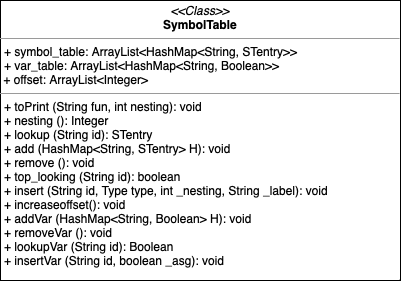
\includegraphics[width=1\linewidth]{Images/ST_structure.png}
  \caption{Struttura della classe SymbolTable}
  \label{fig:STstructure}
\end{subfigure}
\begin{subfigure}{.45\textwidth}
  \centering
  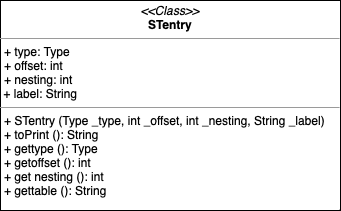
\includegraphics[width=1\linewidth]{Images/STentry _structure.png}
  \caption{Struttura della classe STentry}
  \label{fig:STentrystructure}
\end{subfigure}
\end{figure}

La struttura di STentry contiene i metodi e i campi mostrati in Figura \ref{fig:STentrystructure}, dove:
\begin{itemize}
    \item \textbf{type} è il tipo della varibile o della funzione, dove nel primo caso i tipi ammessi sono int, bool e void, mentre nel secondo caso ho un un tipo \textit{ArrowType} costruito nel modo seguente. Dove \textit{inputtype} è la lista che contiene i tipi dei parametri in input e \textit{outputtype} è il tipo dell'output della funzione, che può essere anch'esso int, bool e void.
    \begin{minted}[xleftmargin=20pt,linenos]{java}
    public class ArrowType extends Type {
	   private ArrayList<Type> inputtype; 
	   private Type outputtype;
    ...
    }
    \end{minted}
    \item \textbf{offset} è un numero intero che indica l'offset di quella variabile o funzione in quell'ambiente.
    \item \textbf{nesting} è un numero intero che indica il livello di nesting nella quale la variabile o funzione è stata dichiarata.
    \item \textbf{label} è una stringa che, nel caso delle variabili è vuota (""), nel caso delle funzioni contiene l'etichetta assegnata a quella funzione da utilizzare in fase di code generation.
\end{itemize}

Per quanto riguarda gli oggetti \textit{$var_table$} e \textit{offset} servono a gestire rispettivamente le variabili dichiarate ma non assegnate e l'assegnamento degli offset. Più informazioni riguardanti la Var Table (VT) sono presenti nella Sezione \ref{sec:vartable}.

Di seguito viene mostrato un esempio del funzionamento della ST.

\begin{minted}[xleftmargin=20pt,linenos]{java}
int a ;
int b ;
int g(int p){
    int y ;
    y = 2;
    p+y
}
int f(int n){
    int b ;
    b = 3;
    g(b+n)
}
a = 1;
b = 2 ;
f(a) ;
\end{minted}

\begin{figure}[h]
\centering
\begin{subfigure}{.23\textwidth}
  \centering
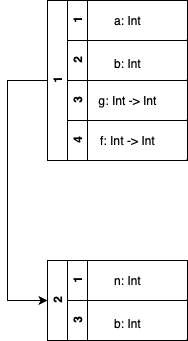
\includegraphics[width=1\linewidth]{Images/ST_example1.png}
  \caption{Symbol table}
\end{subfigure}
\begin{subfigure}{.23\textwidth}
  \centering
  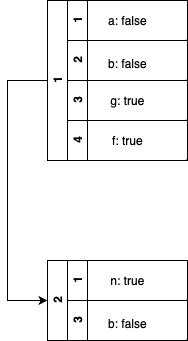
\includegraphics[width=1\linewidth]{Images/VT_example1.png}
  \caption{Var table}
  \label{fig:VTexample}
\end{subfigure}
\caption{ST e VT alla riga 10}
\label{fig:example}
\end{figure}

La ST e VT riga 10 sono mostrate in Figura \ref{fig:example}. Da questa immagine è possibile notare che alle dichiarazioni di funzioni, i loro identificatori vengono salvati nell'ambiente in cui queste vengono dichiarate (in questo caso abbiamo \textit{g} e \textit{f} nell'ambiente 0), quando si entra nel corpo di una funzione viene creato un nuovo ambiente contenente i parametri formali (in questo caso la variabile intera \textit{n}) e gli identificatori degli elementi dichiarati nel corpo della funzione (in questo caso \textit{x}). 

È inoltre utile notare come gli offset siano assegnati agli elementi della ST, il meccanismo è quello di assegnare un valore intero incrementale a partire da 0 in ogni ambiente. Nell'ambiente creato al corpo della funzione verranno prima assegnati i parametri formali, lasciato un offset per il valore di ritorno e solo in seguito vengono assegnati gli elementi dichiarati nel corpo della funzione. 


\subsection{Dichiarazioni multiple}
Per quanto riguarda la gestione degli elementi non dichiarati o dichiarazioni multiple nello stesso ambiente vengono fatti dei controlli durante le dichiarazioni di varibili, funzioni e parametri formali di una stessa funzione.
Nel primo caso si controlla che l'dentificativo utilizzato per la nuova varibile non sia già presente nell'ultimo ambiente della ST (in questo caso viene riportato l'errore), se così non fosse l'identificativo viene aggiunto all'ultimo ambiente della ST. Il controllo è implementato nel nodo \textit{DecvarNode} come segue.
\begin{minted}[xleftmargin=20pt,linenos]{java}
if (ST.top_lookup(id) == true)
        errors.add(new SemanticError("Var id " + id + " already declared"));
    else{
        ST.insert(id, (Type) type, nesting,"") ;
        ST.insertVar(id);
    }
\end{minted}

Nel caso del controllo sulla dichiarazione di funzione e dei suoi paramenti, il controllo eseguito nel nodo \textit{DecfunNode} è il seguente.
\begin{minted}[xleftmargin=20pt,linenos]{java}
if (ST.lookup(id) != null)
    errors.add(new SemanticError("Identifier " + id + " already declared"));
else {
    HashMap<String, STentry> HM = new HashMap<String, STentry>();
    flabel = SimpLanlib.freshFunLabel();
    ST.insert(id, type, nesting, flabel);
    ST.add(HM);
    for (ParNode arg : parlist) {
        if (ST.top_lookup(arg.getId()))
            errors.add(new SemanticError("Parameter id " + arg.getId() +
            " already declared"));
        else {
            ST.insert(arg.getId(), arg.getType(), nesting + 1, "");
        }
    }
    ...
\end{minted}
Come nel caso della dichiarazione di variabile, anche qua si controlla che l'identificativo della funzione non sia presente nell'ultimo ambiente della ST (in questo caso viene riportato l'errore), se così non fosse l'identificativo viene aggiunto all'ultimo ambiente della ST. Solo in seguito viene creato un nuovo ambiente e vengono effettuati i controlli sui paramentri, se questi non sono presenti nell'ultimo (nuovo) ambiente allora vengono aggiunti, altrimenti viene restituito errore. 

\subsection{Identificativi non dichiarati}
Per la gestione degli identificativi non dichiarati sono stati implementati dei controlli sui nodi che richiamano variabili o funzioni, ovvero nel momento in cui viene fatto un assegnamento, espressione che include identificativi o chiamate una fuzione.

Per quanto riguarda il primo caso, il controllo è il seguente e si trova nel nodo \textit{AsgNode}. 
\begin{minted}[xleftmargin=20pt,linenos]{java}
STentry tmp = ST.lookup(id) ;
    if (tmp != null) {
        entry = tmp ; //Se è stato dichiarato allora ok prendo l'entry
    } else { //Se non è stato dichiarato allora errore
        errors.add(new SemanticError("Id " + id + " not declared")) ;
    }
\end{minted}
Prima si recupera l'elemento con identificativo \textit{id} dalla ST, in seguito si controlla se questo elemento sia \textit{null} o meno, nel primo caso si sta provando ad assegnare un'espressione a un elemento non dichiarato, in caso contrario restituisco l'elemento.
Per quanto riguarda le espressioni, bisogna eseguire il controllo nel nodo stesso della variabile, ovvero \textit{IdExpNode}. 
Stessa cosa riguarda la chiamata di funzione, il controllo viene fatto nel nodo \textit{CallNode}. In entrambi i casi, il codice è pressochè simile a quello mostrato precedentemente quindi per semplicità non verrà qui riportato.








%\begin{figure}[h]
%\centering
%\begin{subfigure}{.23\textwidth}
%  \centering
%  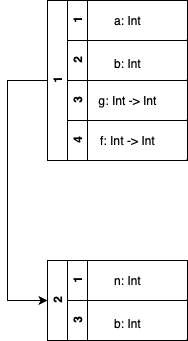
\includegraphics[width=1\linewidth]{Images/ST_example1.png}
%  \caption{Symbol table}
%\end{subfigure}
%\begin{subfigure}{.23\textwidth}
%  \centering
%  \includegraphics[width=1\linewidth]{Images/VT_.png}
%  \caption{Var table}
%\end{subfigure}
%\caption{ST e VT alla riga 9}
%\label{fig:example}
%\end{figure}
\section{Esercizio 3}
Lo scopo dell'esercizio 3 è quello di soddisfare i seguenti punti.
\begin{itemize}
    \item correttezza dei tipi (in particolare numero e tipo dei parametri attuali se conformi al numero e tipo dei parametri formali).
    \item gestione dell'uso di variabili non inizializzate.
\end{itemize}

Una volta implementate le funzionalità della Symbol table, si è proseguito nel progetto lavorando sull’analisi semantica, ovvero verificare la correttezza dei tipi (type checking)  e l’uso di variabili dichiarate ma non inizializzate.

\subsection{Varibili utilizzate ma non inizializzate e Var Table}
\label{sec:vartable}
Prima di proseguire con le modalità di gesitone delle variabili dichiarate ma non inizializzate, è fondamentale fornire più informazioni riguardanti l'utilizzo della Var table utilizzata a questo scopo. Come è stato già introdotta nella Sezione \ref{sec:symboltable}, la Var table (VT) è un elemento della classe \textit{SymbolTable} della forma \textit{$ArrayList<HashMap<String,Boolean>>$}. 

La necessità dell'utilizzo di tale struttura è nato dal momento in cui si è sentita la necessità di voler prendere nota di quali identificatori fossero stati inizializzati e quali no. Come primo approccio c'è stato un tentativo di integrale una variabile \textit{assigned} di tipo bool alla struttura \textit{STentry}, senza però putroppo aver riscontrato buorni risultati. In seguito viene mostrato un esempio di codice che mostra una delle criticità riscontrate.
\begin{minted}[xleftmargin=20pt,linenos]{java}
int x ; 
int y ;
if (e) {
    x = 2 ;
} else {
    y = x ;
}
\end{minted}
Il primo approccio tentato avrebbe previsto l'assegnamento della variabile \textit{assigned = true} alla riga 4 del codice, per poi valutatre come lecita la riga di codice a riga 6, nonostante l'assegnamento fosse stato fatto nel ramo then, uno scope che rimane chiuso tra le due parentesi graffe a riga 3 e 5. In questo codice, la variabile \textit{x} dovrebbe risultare come utilizzata ma non inizializzata.

\begin{minted}[xleftmargin=20pt,linenos]{java}
int x ; 
int y ;
if (e) {
    y = 2 ;
} else {
    x = 1 ;
}
y = x ;
\end{minted}
Secondo il primo approccio tentato, la variabile \textit{x} sarebbe stata assegnata a riga 6, anche qua, in uno scope che diverso rispetto alla quale questa è utilizzata a riga 8. In questo codice, la variabile \textit{x} dovrebbe risultare come utilizzata ma non inizializzata.

Per ricorrere a questo problema, si è deciso di utilizzate una struttura separata da quella della della gestione della ST e quindi avere la possibilità di manipolare gli ambienti di scope delle variabili in modo coerente con la struttura e i nodi del codice. Ciò nonostante la struttura della VT è pressochè simile a quello della ST, difatti entrambe vengono modificate negli stessi punti del codice effettuando le stesse operazioni fatta eccezione dei nodi in cui bisogna effettuare controlli sull'utilizzo delle variabili. Un esempio di come si dovrebbe comportare la VT è presente in Figura \ref{fig:VTexample}. La VT quindi crea/elimina nuovi "scope" nello stesso momento in cui sulla ST vengono creati/eliminati nuovi ambienti. Le uniche eccezioni e controlli aggiuntivin vengono applicati nei nodi del condizionale if, sia \textit{IfExpNode} che \textit{IfStmNode}, il nodo dell'assegnamento \textit{AsgNode} e il nodo foglia degli id \textit{IdExpNode}. I codici risultati sono i seguenti.
\begin{minted}[xleftmargin=20pt,linenos]{java}
public ArrayList<SemanticError> checkSemantics(SymbolTable ST, int _nesting) {
        nesting = _nesting;
        ArrayList<SemanticError> errors = new ArrayList<SemanticError>();
        errors.addAll(exp.checkSemantics(ST, nesting));
        HashMap<String, Boolean> V1 = new HashMap<String,Boolean>() ;
        ST.addVar(V1);
        for (Node d : thenbranch) {
            errors.addAll(d.checkSemantics(ST, nesting)) ;
        }
        ArrayList<String> V1List = TakeDeclaredVariables(V1);
        ST.removeVar();
        HashMap<String, Boolean> V2 = new HashMap<String,Boolean>() ;
        ST.addVar(V2);
        for (Node d : elsebranch) {
            errors.addAll(d.checkSemantics(ST, nesting)) ;
        }
        ArrayList<String> V2List = TakeDeclaredVariables(V2);
        ST.removeVar();
        ArrayList<String> FinalList= CompareEnvironmentVariables(V1List, V2List);
        for (String id: FinalList)
            ST.insertVar(id, true);
        return errors;
    }
\end{minted}
Il codice soprastante è quello utilizzato nelle classi \textit{IfExpNode} che \textit{IfStmNode}. In questo caso, a riga 7 e 14 vengono dichiarati due nuove strutture \textit{$HashMap<String, Boolean>$} utilizzate per tenere traccia delle variabili inizializzate corrispettivamente nel ramo then ed else. A riga 12 e 19, viene utilizzata la funzione \textit{$TakeDeclaredVariables(HashMap<String, Boolean> V)$} per mettere in una lista \textit{$ArrayList<String>$} il nome delle variabili inizializzate in quello scope. Solo a riga 21 la funzione  \textit{$CompareEnvironmentVariables(ArrayList<String> L1, ArrayList<String> L2)$} compara le due liste e a riga 23 gli elementi presenti in entrambe le liste vengono aggiunte allo scope attuale. Tramite questa tecnica è possibile risolvere i problemi mostrati precedentemente dal momento in cui veongo creati e distrutti scope apposta per i due rami dell'if senza andare a modificare direttamente lo socpe attuale.

Ma come è possibile sapere se un identificativo è stato assegnato o meno nel momento in cui viene eseguita un'espressione o statement? Nel nodo \textit{IdExpNode} è stato aggiunto il seguente controllo.
\begin{minted}[xleftmargin=20pt,linenos]{java}
//Controllo se è assegnato nella tabella degli assegnamenti
Boolean varInfo = ST.lookupVar(id) ; 
if(varInfo!= null)
    if(varInfo == FALSE && (st_type.getnesting() == nesting)){ 
    //Se la variabile non è assegnata
    errors.add(new SemanticError("Id " + id + " used but not initialized"));
}
\end{minted}
Tramite questo controllo è possibile ottenere tramite la funzione \textit{lookupVar(String id)} l'oggetto nella VT che fa riferimento all'id \textit{id}. A riga 3 viene verficato che l'elemento esista, in questo caso è stato dichiarato e aggiunto alla tablla correttamente. Dopo di che viene controllato a riga 4 se l'elemento è presente in questo scope e ha come valore FALSE allora non è mai stato inizializzato e deve essere restituito un errore.

È inoltre importante precisare che nel momento in cui l'id delle funzioni viene aggiunto alla VT, questo avrà sempre valore TRUE per fare in modo che nel corpo di una funzione, questa possa richiamare sè stessa pur appartenendo allo stesso scope. Stessa cosa avviene per i parametri formali delle funzioni, anch'essi vengono assegnati come TRUE dal momento in cui vengono inizializzati durante la chiamata a funzione. In fine, nel momento in cui viene fatto un assegnamento, l'identificativo di sinista viene aggiunto alla VT con valore TRUE.

\subsection{Regole di inferenza}
Per quanto riguarda il type cheking sono state specificate le seguenti regole di inferenza dove:
\begin{itemize}
    \item L'ambiente $\Gamma$ è una funzione definita come $\Gamma:ID \rightarrow type, O, nesting $ e fa riferimento alla ST.
    \item Lo scope $\Theta$ è una funzione definita come $\Theta:ID \rightarrow assigned$ e fa riferimento alla VT.
\end{itemize}

\subsubsection{Progammi}
\textbf{Programma solo con espressione}
\[
\inference{\emptyset \cdot [], \emptyset \cdot [], O, N \vdash exp:\Gamma, \Theta, T}{ \vdash exp: T }[[ProgExp]]
\]
Regola iniziale del programma che contiene solo un espressione. L'offset e il livello di nesting iniziale viene posto a 1. \\

\textbf{Programma con dichiarazioni, statement ed espressione}
\[
\inference{\emptyset \cdot [], \emptyset \cdot [], O, N \vdash dec:\Gamma, \Theta \\ \Gamma, \Theta \vdash stm:\Gamma, \Theta^{'} \\ \Gamma, \Theta^{'} \vdash exp:\Gamma, \Theta^{''}, T}{ \vdash dec \; stm \; exp}[[Prog1]]
\]
Regola iniziale del programma, consente di avere dichiarazioni, statements e un'epressione. L'offset e il livello di nesting iniziale viene posto a 1. \\

\textbf{Programma con dichiarazioni ed espressione}
\[
\inference{\emptyset \cdot [], \emptyset \cdot [], O, N \vdash dec:\Gamma, \Theta \\ \Gamma, \Theta \vdash exp:\Gamma, \Theta^{'}, T}{ \vdash dec \; exp}[[Prog2]]
\]
Regola iniziale del programma, consente di avere dichiarazioni e un'epressione. L'offset e il livello di nesting iniziale viene posto a 1. \\

\subsubsection{Dichiarazioni}
\textbf{Dichiarazione di variabile}
\[
\inference{id \notin dom(top(\Gamma))}{\Gamma, \Theta, O \vdash T \; id;: \Gamma[id \rightarrow T], \Theta[id \rightarrow false] , O+1}[[DecVar]]
\]
Nella dichiarazione di variabile bisogna controllare che l'identificativo non faccia parte dell'ultimo ambiente di $\Gamma$, in caso contrario l'id viene aggiunto all'ambiente $\Gamma$ e scope $\Theta$ attuale. Nello scope $\Theta$, l'identificatore della variabile viene assegnata a false perché non è ancora stata inizializzata. L'offset $O$ viene incrementato di 1 per fare riferimento alla variabile nello stack.\\

\textbf{Sequenza di dichiarazioni}
\[
\inference{\Gamma, \Theta, O \vdash d:\Gamma^{'}, \Theta^{'}, O^{'} & \Gamma^{'}, \Theta^{'}, O^{'} \vdash D:\Gamma^{''}, \Theta^{''}, O^{''} }{\Gamma, \Theta, O \vdash d \; D: \Gamma^{''}, \Theta^{''}}[[DecSeq]]
\]
Nella sequenza di dichiarazioni viene esplorata una dichiarazione alla volta. L'ambiente, lo scope e l'offset vengono aggionati dopo la prima dichiarazione e quindi vengono passati alle dichiarazioni che seguono la prima. \\

\textbf{Dichiarazione di funzione}
\[
\inference{\Gamma \cdot [f \mapsto(argsTypes(args)) \rightarrow T], \Theta \cdot[f \mapsto true], O+1, N+1 \vdash args: \Gamma^{'}, \Theta^{'}, O^{'}, N^{'} \\ \Gamma^{'}, \Theta^{'}, O^{'}+1 , N^{'}\vdash body: T1 \\ f \notin dom(top(\Gamma)) & T= T1}{\Gamma, \Theta, O, N \vdash T \; f(args)\{body\} : \Gamma [f \mapsto(argsTypes(args)) \rightarrow T], \Theta [f \mapsto true]}[[DecFun]]
\]
Nella dichiarazione di funzione viene creato un nuovo ambiente in $\Gamma$ e un nuovo scope in $\Theta$. L'oggetto $args$ è costruito nel modo seguente $T_{1} x_{1}, ..., T_{n} x_{n}$. In $\Gamma$ viene aggiunto l'id della funzione che ha come tipo un oggetto costrutito come $(T_{1},..., T_{n}) \rightarrow T$, ovvero "i tipi dei parametri in input" $\rightarrow$ "il tipo della funzione". Per ottenere il tipo dei parametri $T_{1},..., T_{n}$ viene usata la funzione \textit{argsTypes(args)}. In $\Theta$ viene aggiunto l'identificativo della funzione con valore true per fare in modo che questo possa essere richiamato nell corpo della funzione stessa. Nella regola che va in arg, l'offset $O$ viene incrementato di 1 perché si stanno valutando elementi interni a un nuovo ambiente e scope, inoltre, anche il livello di nesting $N$ aumenta di 1 per fare riferimento all'identificativo della funzione nello stack. Nella regola che va nel body l'offset $O^{'}$ viene incrementato nuovamente per fare spazio all'indirizzo di ritorno. \\
%Nel nuovo ambiente $\Gamma$, vengono inoltre aggiunti tutti gli id dei parametri e il loro tipo. 

\textbf{Parametro (un argomento)}
\[
\inference{id \notin dom(top(\Gamma))}{\Gamma, \Theta, O \vdash T \; id: \Gamma[id \rightarrow T], \Theta[id \rightarrow true] , O+1}[[Arg]]
\]
Se l'identificativo del parametro non appartiene all'ultimo ambiente $\Gamma$ allora lo si aggiunge all'ultimo ambiente $\Gamma$, gli viene assegnato nello scope $\Theta$ il valore true e l'offset viene aumentato di 1. \\

\textbf{Parametri (argomenti di funzione)}
\[
\inference{\Gamma, \Theta, O \vdash a: \Gamma^{'}, \Theta{'}, O^{'} \\ \Gamma^{'}, \Theta^{'}, O^{'} \vdash A: \Gamma^{''}, \Theta{''}, O^{''} }{\Gamma, \Theta, O \vdash a \; A: \Gamma^{''}, \Theta{''}, O^{''} }[[Args]]
\]

\textbf{Dichiarazioni, statement ed espressione (Body)}
\[
\inference{\Gamma, \Theta, O \vdash dec:\Gamma^{'}, \Theta, O^{'} \\ \Gamma^{'}, \Theta, O^{'} \vdash stm:\Gamma^{'}, \Theta^{'}, O^{'} \\ \Gamma^{'}, \Theta^{'}, O^{'} \vdash exp:\Gamma^{'}, \Theta^{''}, O^{'}, T}{\Gamma, \Theta \vdash dec \; stm \; exp: T}[[Body]]
\]

\subsubsection{Statements}
\textbf{Assegnamento}
\[
\inference{\Gamma, \Theta, N \vdash Id:T1 & \Gamma, \Theta \vdash exp:\Gamma, \Theta^{'}, T2 \\ T1 = T2}{\Gamma, \Theta, N \vdash Id \; = \; exp: \Gamma, \Theta^{'}[Id\mapsto true], void}[[Asg]]
\]
Viene controllato che i tipi dell'identificativo e dell'espressione siano gli stessi. Nello scope $\Theta$ l'identificativo viene assegnato a true in seguito all'assegnamento. \\

\textbf{Condizionale if (stm)} 
\[
\inference{\Gamma, \Theta \vdash exp:\Gamma, \Theta^{'}, T1 & \Gamma, \Theta^{'} \vdash stme1:\Gamma, \Theta^{''}, T2 & \Gamma, \Theta^{'} \vdash stme2:\Gamma, \Theta^{'''}, T3 \\ T1 = bool }{\Gamma, \Theta \vdash if\; (exp)\; \{ stme1 \}\; else\; \{stme2\}: \Gamma, CompScope(\Theta^{''}, \Theta^{'''}), void}[[IfStm1]]
\]
Nel condizionale if bisogna innanzitutto controllare che l'espressione della condizione sia di tipo booleano. I due rami alterano lo scope $\Theta$ in modo diverso, ragione per cui viene utilizzata una funzione $CompScope(\Theta^{''}, \Theta^{'''})$ per paragonare i due nuovi scope e passare lo scope di ritorno contenente gli identificativi valutati come assegnati in modo corretto. Tale funzione compara i due scope tenendo traccia di quali identificativi siano assegnati come true, se questi sono presenti in entrambi gli scope allora rimangono, altrimenti le modifiche vengono riportate a $\Theta^{'}$.\\

\textbf{Condizionale if senza ramo else (stm)} 
\[
\inference{\Gamma, \Theta \vdash exp:\Gamma, \Theta^{'}, T1 & \Gamma, \Theta^{'} \vdash stme1:\Gamma, \Theta^{''}, T2 \\ T1 = bool}{\Gamma, \Theta \vdash if\; (exp)\; \{ stme1 \}: \Gamma, \Theta^{'}, void}[[IfStm2]]
\]

\textbf{Statement}
\[
\inference{\Gamma, \Theta \vdash s:\Gamma, \Theta^{'}, T }{\Gamma, \Theta \vdash s \; S: \Gamma, \Theta^{''}, void}[[Stm]]
\]

\textbf{Sequenza di statements}
\[
\inference{\Gamma, \Theta \vdash s:\Gamma, \Theta^{'}, T1 & \Gamma, \Theta^{'} \vdash S:\Gamma, \Theta^{''}, T2 }{\Gamma, \Theta \vdash s \; S: \Gamma, \Theta^{''}, void}[[SeqStm]]
\]

\textbf{Chiamata di funzione} 
\[
\inference{\Gamma, \Theta \vdash f: (T_{1}, ..., T_{n}) \rightarrow T & (\Gamma e_{i}: T^{'}_{i})^{n}_{i = 1} & (T_{i} = T^{'}_{i})^{n}_{i = 1}}{\Gamma, \Theta \vdash f(e_{1},...,e_{n});: \Gamma, \Theta, T}[[CallExp]]
\]
Si controlla che i parametri attuali e formali in input alla funzione abbiamo un tipo compatibile. \\

\subsubsection{Espressioni}

\textbf{Espressione generica}
\[
\inference{\Gamma, \Theta \vdash exp:\Gamma, \Theta^{'}, T}{\Gamma, \Theta \vdash exp: \Gamma, \Theta^{''}, T}[[Exp]]
\]

\textbf{Assioma intero} 
\[
\inference{}{\Gamma \vdash num: \Gamma, int}[[IntExp]]
\]

\textbf{Assioma booleano} 
\[
\inference{}{\Gamma \vdash true: \Gamma, bool}[[BoolExpTrue]]
\]
\[
\inference{}{\Gamma \vdash false: \Gamma, bool}[[BoolExpFalse]]
\]

\textbf{Variabile} 
\[
\inference{id \in dom(\Gamma): T \\ (\Theta(id) = true \lor \neg(\Gamma(id).nesting = N))}{\Gamma, \Theta, N \vdash id:  T}[[IdExp]]
\]
In questo caso bisogna controllare che l'identificativo della variabile sia presente in $\Gamma$ e che il valore dell'identificatico in $\Theta$ sia true (ovvero la variabile è assegnata) oppure che non sia stata dichiarata nell'ambiente attuale (e quindi in quel caso è una variabile globale e deve essere accettata). 

\textbf{Espressione in parentesi} 
\[
\inference{\Gamma, \Theta \vdash exp: \Gamma, \Theta^{'}, T}{\Gamma, \Theta \vdash (exp): \Gamma, \Theta^{'}, T}[[BaseExp]]
\]

\textbf{Espressioni booleane} 
\[
\inference{\Gamma, \Theta \vdash exp: \Gamma, \Theta^{'}, T & T==bool}{\Gamma, \Theta \vdash !\; exp: \Gamma, \Theta^{'}, bool}[[NotExp]]
\]

\[
\inference{\Gamma, \Theta \vdash e1:\Gamma, \Theta^{'}, T1 & \Gamma, \Theta^{'} \vdash e2:\Gamma, \Theta^{''}, T2 \\ T1 = bool = T2 & \sigma: bool \times bool \rightarrow bool}{\Gamma, \Theta \vdash e1 \; \sigma \; e2: \Gamma, \Theta^{''}, bool}[[OpExp]]
\]
Dove il simbolo $\sigma$ viene utilizzato per fare riferimento ai simboli:$\&\&$ e $||$. \\

\textbf{Espressioni intere} 
\[
\inference{\Gamma, \Theta \vdash e1:\Gamma, \Theta^{'}, T1 & \Gamma, \Theta^{'} \vdash e2:\Gamma, \Theta^{''}, T2 \\ T1 = int = T2 & \sigma: int \times int \rightarrow int}{\Gamma, \Theta \vdash e1 \; \sigma \; e2: \Gamma, \Theta^{''}, int}[[NumExp]]
\]
Dove il simbolo $\sigma$ viene utilizzato per fare riferimento ai simboli:$+, -, *$ e $/$. \\

\textbf{Espressioni di confronto} 
\[
\inference{\Gamma, \Theta \vdash e1:\Gamma, \Theta^{'}, T1 & \Gamma, \Theta^{'} \vdash e2:\Gamma, \Theta^{''}, T2 \\ T1 = T2 & ==: T1 \times T2 \rightarrow bool}{\Gamma, \Theta \vdash e1 \; == \; e2: \Gamma, \Theta^{''}, bool}[[EqExp]]
\]

\[
\inference{\Gamma, \Theta \vdash e1:\Gamma, \Theta^{'}, T1 & \Gamma, \Theta^{'} \vdash e2:\Gamma, \Theta^{''}, T2 \\ T1 = int = T2 & \sigma: int \times int \rightarrow bool}{\Gamma, \Theta \vdash e1 \; \sigma \; e2: \Gamma, \Theta^{''}, bool}[[NumExp]]
\]
Dove il simbolo $\sigma$ viene utilizzato per fare riferimento ai simboli:$<, <=, >$ e $>=$. \\


\textbf{Condizionale if (exp)} 
\[
\inference{\Gamma, \Theta \vdash cond:\Gamma, \Theta^{'}, T1 & \Gamma, \Theta^{'} \vdash stme1:\Gamma, \Theta^{''}, T2 & \Gamma, \Theta^{''} \vdash stme2:\Gamma, \Theta^{'''}, T3 \\ T1 = bool & T2 = T = T3}{\Gamma, \Theta \vdash if\; (cond)\; \{ stme1 \}\; else\; \{stme2\}: \Gamma, CompScope(\Theta^{''}, \Theta^{'''}), T}[[IfExp]]
\]
Anche in questo caso, come nel caso del condizionale if (stm) senza espressione, bisogna controllare che la condizione sia di tipo booleano ed anche qua viene utilizzata la funzione $CompScope(\Theta^{''}, \Theta^{'''})$ per comparare gli scope dei due branch. \\

\textbf{Statement ed espressione}
\[
\inference{\Gamma, \Theta \vdash stm:\Gamma, \Theta^{'}, T1 & \Gamma, \Theta^{'} \vdash exp:\Gamma, \Theta^{''}, T2 \\ T1 = void}{\Gamma, \Theta \vdash stm \; exp: \Gamma, \Theta^{''}, T2}[[StmExp]]
\]

\textbf{Chiamata di funzione} 
\[
\inference{\Gamma, \Theta \vdash f: (T_{1}, ..., T_{n}) \rightarrow T & (\Gamma e_{i}: T^{'}_{i})^{n}_{i = 1} & (T_{i} = T^{'}_{i})^{n}_{i = 1}}{\Gamma, \Theta \vdash f(e_{1},...,e_{n}): \Gamma, \Theta, T}[[CallExp]]
\]


\subsection{Esempi}
In questa sezione testiamo i seguenti 4 codici forniti nelle specifiche del progetto.
\begin{enumerate}
\item \textbf{Codice 1}
\begin{minted}[xleftmargin=20pt,linenos]{java}
int a;
int b;
int c ;
c = 2 ;
if (c > 1) {
    b = c ; 
} else {
    a = b ;
}
\end{minted}
I messaggi in output dal compilatore sono i seguenti.
\begin{minted}[xleftmargin=20pt,linenos]{java}
Parsing in progress....
Parse completed without errors!
Checking semantic errors...
You had: 1 errors:
[!] A semantic error occurred: Id b used but not initialized	
\end{minted}
Come si legge dallì'ultimo messaggio di errore, l'identificatore \textit{b} è utilizzato ma mai usato, infatti è possibile vedere che nel ramo then b è effettivamente inizializzato ma tale modifica è presente e valida solo in quel ramo, quindi una volta che il compilatore controlla gli elementi utilizzati nell'espressione del ramo else, trova errore a riga 8 nel momento in cui si prova a utilizzare \textit{b}, dichiarato a riga 2 ma mai inizializzato in questo scope.

\item \textbf{Codice 2}
\begin{minted}[xleftmargin=20pt,linenos]{java}
int a ; 
int b ; 
int c ;
void f(int n){
    int x ; 
    int y ;
    if (n > 0) {
        x = n ;
    } else {
        y = n+x ;
    }
 }
 c = 1 ;
 f(0) ;
\end{minted}
I messaggi in output dal compilatore sono i seguenti.
\begin{minted}[xleftmargin=20pt,linenos]{java}
Parsing in progress....
Parse completed without errors!
Checking semantic errors...
You had: 1 errors:
[!] A semantic error occurred: Id x used but not initialized	
\end{minted}
Anche in questo caso, come nel caso precedente, il compilatore segnala un uso illecito della variabile \textit{x}, questa è inizializzata nel corpo della funzione \textit{f} a riga 5 e inizializzata nel ramo then, quindi nel momento in cui il controllo raggiunge il ramo else l'id \textit{x} non risulta inizializzato in questo scope.

\item \textbf{Codice 3}
\begin{minted}[xleftmargin=20pt,linenos]{java}
void h(int n){
    int x ;
    int y ;
    if (n==0){
        x = n+1 ;
    } else {
    h(n-1) ; 
    x = n ; 
    y = x ;
    }
}    
h(5) ;
\end{minted}
I messaggi in output dal compilatore sono i seguenti.
\begin{minted}[xleftmargin=20pt,linenos]{java}
Parsing in progress....
Parse completed without errors!
Checking semantic errors...
Visualizing AST...
Checking type errors...
Type checking ok! Type of the program is: [T]Void
Code generated! Assembling and running generated code.
...
\end{minted}
Eseguedo questo codice non vengono trovati errori da parte del compilatore.

\item \textbf{Codice 4}
\begin{minted}[xleftmargin=20pt,linenos]{java}
int a;
void h(int n){
    int x ;
    int y ;
    if (n==0){
        x = n+1 ;
    } else {
        h(n-1) ;
        y = x ;
    }
}
h(5) ;
\end{minted}
I messaggi in output dal compilatore sono i seguenti.
\begin{minted}[xleftmargin=20pt,linenos]{java}
Parsing in progress....
Parse completed without errors!
Checking semantic errors...
You had: 1 errors:
[!] A semantic error occurred: Id x used but not initialized	
\end{minted}
Anche in questo codice, come in quelli precedenti, il compilatore segnala che la variabile \textit{x} sia stata utilizzata ma non inizializzata, questa è inizializzata nel corpo della funzione \textit{h} a riga 2 e inizializzata nel ramo then, quindi nel momento in cui il controllo raggiunge il ramo else l'id \textit{x} non risulta inizializzato in questo scope.
\end{enumerate}
\section{Esercizio 4}
Lo scopo di questo esercizio è quello di estendere l'interprete di SimpLan per implementare l'interprete di SimpLanPlus. 

\subsection{Interprete SVM}
Per perseguire gli obiettivi di questa fase, è stato importato al progetto il file \textit{SVM.g4}, contentente la grammatica dell'interprete di base, nel package \textit{svm}. In seguito è stato utilizzato lo stesso metodo già utlizzato per la grammatica del compilatore \textit{SimpLanPlus.g4}, ovvero è stato utilizzato ANTLR per generare il codice del visitor della SVM. Successivamente, sono stati creati i metodi per la generazione di codice in ogni nodo dell'albero creato precedentementemente per costruire l'AST. 

Nel main sono state aggiunte le componenti che scrivono in un file di appoggio \textit{prova.simplan.asm} (contenuto nel package \textit{mainPackage}) il codice generato dal programma. Venogno poi utilizzati gli stessi step usati precedentemente per leggere il nuovo file creato, estrarre i token ed effettuare il parser. In fine, viene eseguita la VM per eseguire il codice generato.

\subsection{Esercizi}
In questa sezione testiamo i seguenti 4 codici forniti nelle specifiche del progetto.

\begin{enumerate}
\item \textbf{Codice 1}
\begin{minted}[xleftmargin=20pt,linenos]{java}
int x ;
void f(int n){
	if (n == 0) { n = 0 ; }       // n e` gia` uguale a 0; equivale a fare skip
	else { x = x * n ; f(n-1) ; }
}
x = 1 ;
f(10)
\end{minted}
Il codice viene compilato ed eseguito correttamente ed il risultato ottenuto è 0 dal momento in cui la funzione chiamata è di tipo void, ovvero non restituisce nessun valore. Il valore di ritorno è salvato nel registro a0 che viene inzialmente settato a 0.

\begin{minted}[xleftmargin=20pt,linenos]{java}
Parsing in progress....
Parse completed without errors!
Checking semantic errors...
Visualizing AST...
Checking type errors...
Type checking ok! Type of the program is: [T]Void
Code generated! Assembling and running generated code.
Starting Virtual Machine...
*** STACK ***
Code executed with success!
The result is: 0
\end{minted}

\item \textbf{Codice 2}
\begin{minted}[xleftmargin=20pt,linenos]{java}
int u ;
int f(int n){
        int y ;
	y = 1 ;
	if (n == 0) { y }
	else { y = f(n-1) ; y*n }
}
u = 6 ;
f(u)
\end{minted}
Il codice viene compilato ed eseguito correttamente ed il risultato ottenuto è 720.

\begin{minted}[xleftmargin=20pt,linenos]{java}
Parsing in progress....
Parse completed without errors!
Checking semantic errors...
Visualizing AST...
Checking type errors...
Type checking ok! Type of the program is: [T]Void
Code generated! Assembling and running generated code.
Starting Virtual Machine...
*** STACK ***
Code executed with success!
The result is: 720
\end{minted}

\item \textbf{Codice 3}
\begin{minted}[xleftmargin=20pt,linenos]{java}
int u ;
void f(int m, int n){
	if (m>n) { u = m+n ;}
	else { int x ; x = 1 ; f(m+1,n+1) ; }
}
f(5,4) ;
\end{minted}
Il compilatore si interrompe al controllo degli errori presenti nel parser nel momento in cui il codice non è coerente con la gammatica. Infatti, nel corpo del ramo else è presente una dichiarazione di variabile. Le dichiarazioni non sono consentite nei branch del costrutto if.

\begin{minted}[xleftmargin=20pt,linenos]{java}
Parsing in progress....
[!] An error occurred at line 4, character 8 :extraneous input 'int' 
expecting {'if', ID}
[!] An error occurred at line 4, character 14 :no viable alternative 
at input 'x;'
parser.ParserErrorHandler@15d0c81b
\end{minted}
\end{enumerate}

% ----------------------------------------------------------------------
% Conclusion
% ----------------------------------------------------------------------
%\section{Conclusion}


% ----------------------------------------------------------------------
% References
% ----------------------------------------------------------------------
%\bibliographystyle{plain}
%\bibliography{refs}

% ----------------------------------------------------------------------
% Appendices
% ----------------------------------------------------------------------
%\appendix  
\clearpage
\addappheadtotoc 
\appendixpage 

\section{First appendix}


\section{Second appendix}

\end{document}